%!TEX encoding = IsoLatin

%% Document is article 
\documentclass[a4paper]{article}

%% ----------------------------------------------------- PACKAGES ----------------------------------------------------- %%
\usepackage{coolArticle}
\usepackage{caption}

%% ---------------------------------------------------- DOCUMENT ---------------------------------------------------- %%
\begin{document}

\noindent \textsc{Gallois-Montbrun} Gr�goire\\
\textsc{Faury} Louis 
	\titlebox{0.6}{Model Predictive Control}{Exercice \#1 - \textcolor{blue}{Group 2}}
	
	\vspace{10pt}
	\paragraph{} We consider the linear discrete-time LTI defined by : 
	\begin{equation}
		\begin{aligned}
			x_{i+1} &= Ax_i + Bu_i \\
			y_i &= Cx_i
		\end{aligned}
	\end{equation} 
	with : 
	\begin{equation}
		A = \begin{bmatrix} \frac{4}{3} & -\frac{2}{3} \\1 & 0\end{bmatrix}, \quad B = \begin{bmatrix} 1 \\ 0 \end{bmatrix} \quad \text{ and } \quad C = \begin{bmatrix} - \frac{2}{3} &  1\end{bmatrix}
	\end{equation}
	We can already state that the \textbf{system is controlable and observable} since the Kalman matrix and the observability matrix both are full rank : 
	\begin{equation}
		\mathcal{C} = \begin{bmatrix}  1& \frac{4}{3} \\ 0 & 1\end{bmatrix}\,, \quad \mathcal{O} = \displaystyle\begin{bmatrix}-2/3 & 1 \\ 1/9 & 4/3\end{bmatrix}
	\end{equation}
	
	Figure (\ref{uncontrolled}) shows the output trajectory of the uncontrolled system (i.e $u=0$). We see that the system is stable which is confirmed by the analysis of matrix $A$. The norm of $\lambda_1$ and $\lambda_2$, its eigenvalues, is inferior to $1$:
	\begin{equation}
		\lambda_1 = 0.6667 + 0.4714i \textrm{	and	    } \lambda_2 = 0.6667 - 0.4714i
	\end{equation}
	
	\begin{figure}[h!]
		\centering
		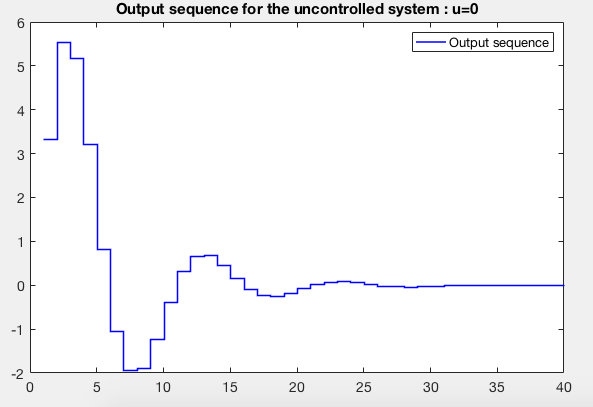
\includegraphics[width=0.5\linewidth]{free_traj}
		\caption{Uncontrolled system output sequence}
		\label{uncontrolled}
	\end{figure}
	
	
	
	\paragraph{} We consider the LQR optimization problem. Given an horizon $N$, it writes : 
	\begin{equation}
		u^* = \min_u{\left\{ V(x,u) = \sum_{i=0}^{N-1} \left[x_i^TQx_i + u_i^TRu_i\right] + x_N^TP_fx_N\right\}}
	\end{equation}
	
	with $Q=C'C + 0.001\mathbb{I}_2$, $P_f=Q$ and $R = 0.001$. 
	\section{Exercise 1}
	{
		\paragraph{} We implemented the discrete-time Riccati recursion to compute the linear feedback law that solves the LQR optimization problem. The update rules are given by, assuming a horizon $N$ : 
		\begin{equation}
			\begin{aligned}
				H_N &= P_f \\
				i=N-1\hdots 0 : \quad 
					&\left\{ \begin{aligned} K_i &= -(R+B^TH_{i+1}B)-B^TH_{i+1}A\\
									H_i &= Q+K_i^TRK_i +(A+BK_i)^TH_{i+1}(A+BK_i)
					\end{aligned}\right.
			\end{aligned}
		\end{equation}
		
		% least square ? 
	}
	
	\section{Exercise 2}
	{
	
		\begin{figure}[h!]
			\begin{minipage}{0.5\linewidth}
				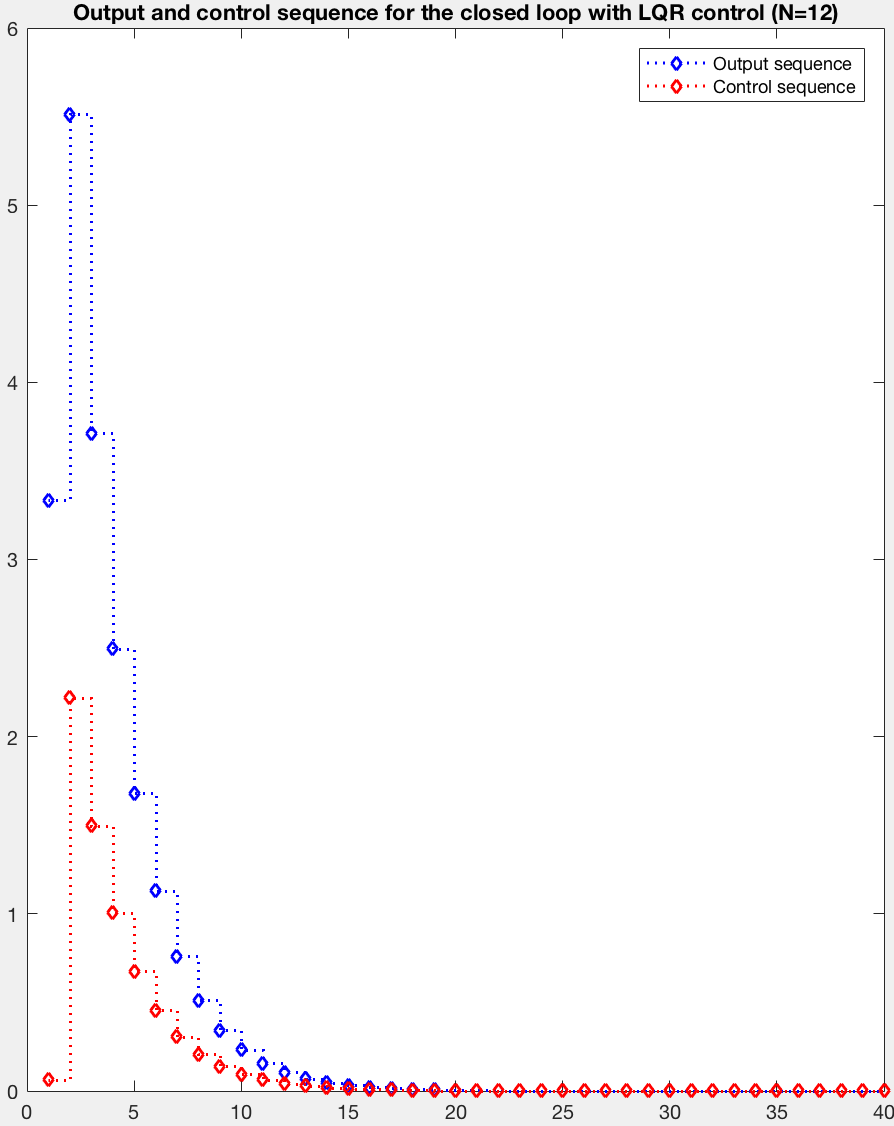
\includegraphics[width=0.9\linewidth]{traj_n12}
				\caption{Output and control sequences for N=12}
				\label{n12}
			\end{minipage}
			\begin{minipage}{0.5\linewidth}
				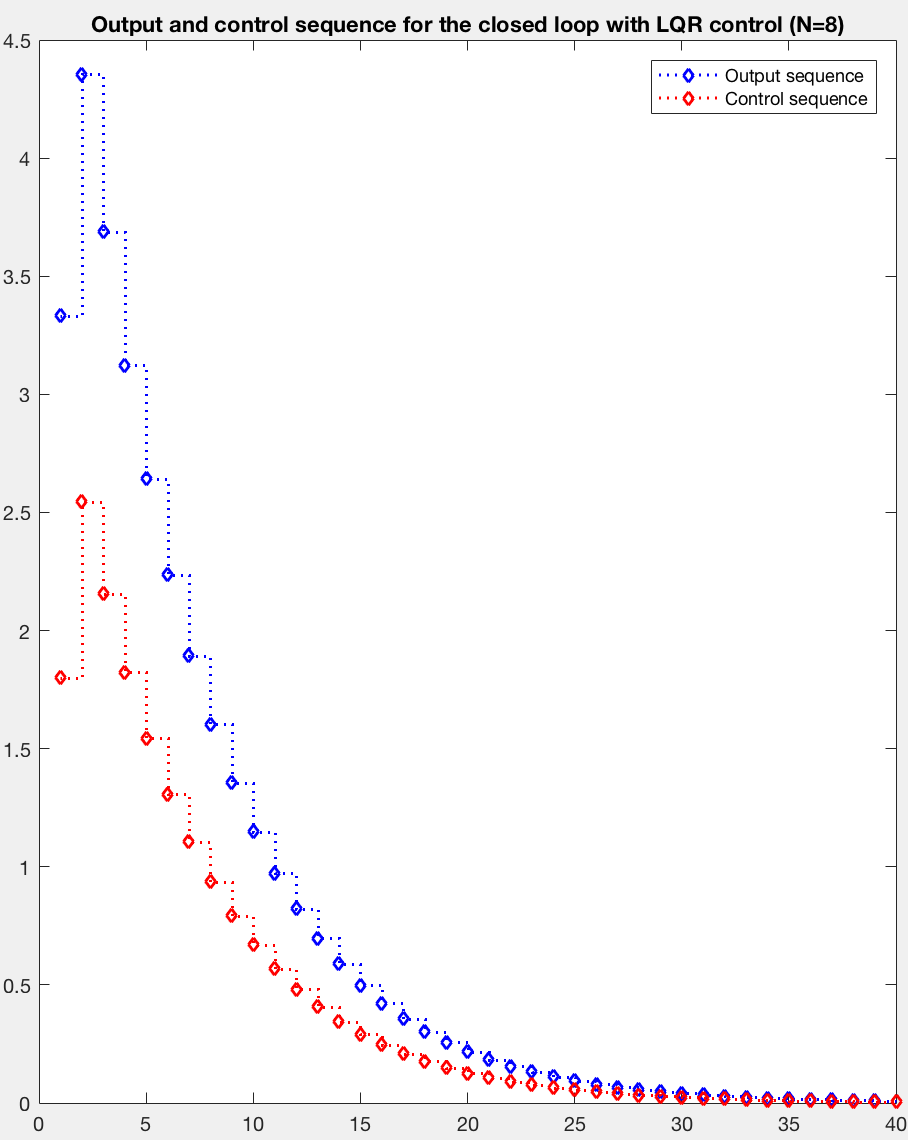
\includegraphics[width=0.9\linewidth]{traj_n8}
				\caption{Output and control sequences for N=8}	
				\label{n8}			
			\end{minipage}
		\end{figure}
		
		\paragraph{} We then implemented the LQR control in a receding horizon fashion, starting at state $x_0 = \begin{bmatrix} 10 \\ 10 \end{bmatrix}$. Computing trajectories for different values of $N$, we can see that \textbf{the minimum horizon length that stabilizes the system is $\color{red} N^* = 7$}. We give a few examples of trajectories on figure (\ref{n12}) and (\ref{n8}).
		
		\paragraph{} We show the results we obtain when plotting predicted trajectories for different values of $N$ on figure (\ref{n7}) and (\ref{n10}). On these figures, dashed lines represent open loop trajectories anticipated by the receding horizon controller while blue lines represent real closed-loop trajectories. By increasing $N$, we see that our open-loop controller computes smoother and more realistic trajectories, as it is able to account for more futur dynamics. We indeed see that the greater the horizon is, the more the open-loop and closed-loop curve fit with one another, as future, possible unstable dynamic is accounted for. 
		
		\begin{figure}[h!]
			\begin{minipage}{0.5\linewidth}
				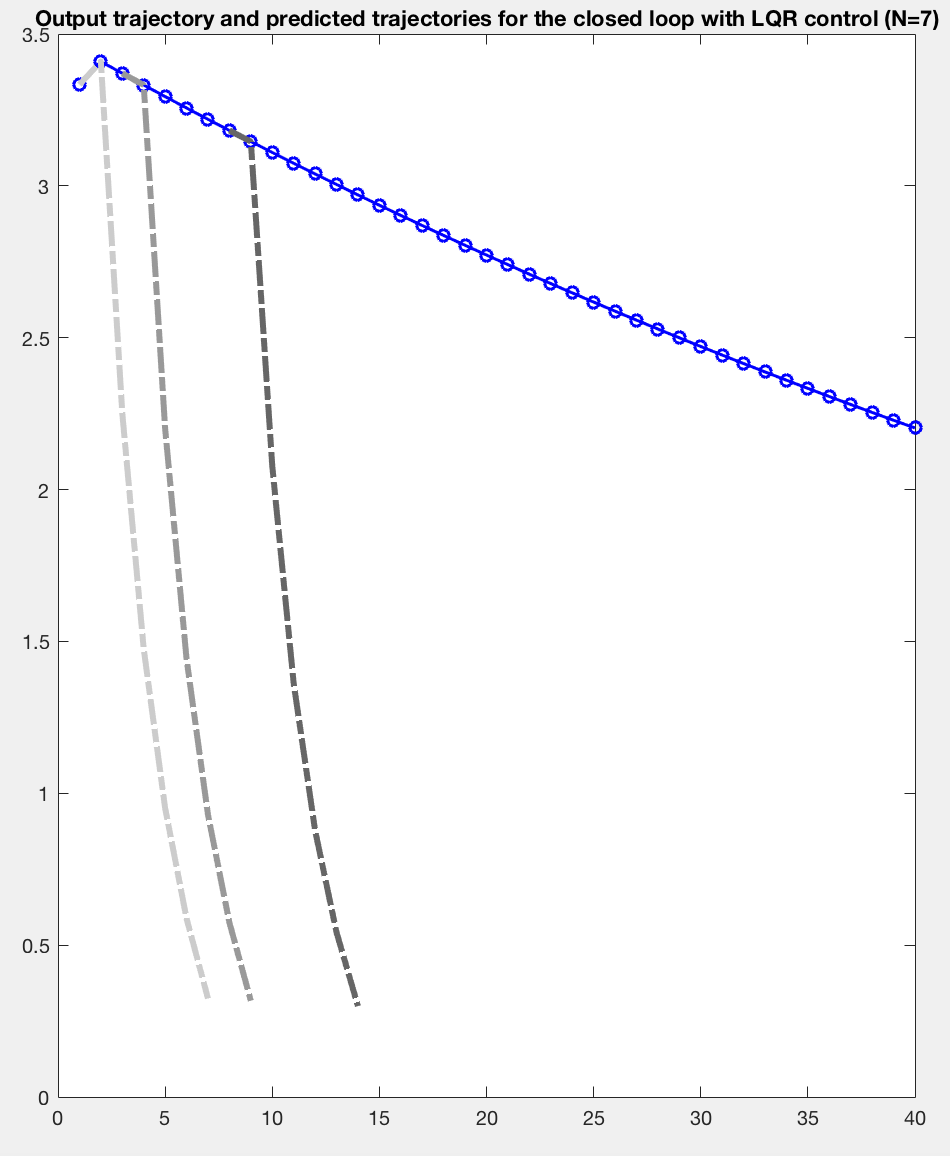
\includegraphics[width=0.9\linewidth]{pred_n7}
				\captionsetup{justification=centering,margin=0.5cm}
				\caption{Predicted and actual output trajectory for N=7}
				\label{n7}
			\end{minipage}
			\begin{minipage}{0.5\linewidth}
				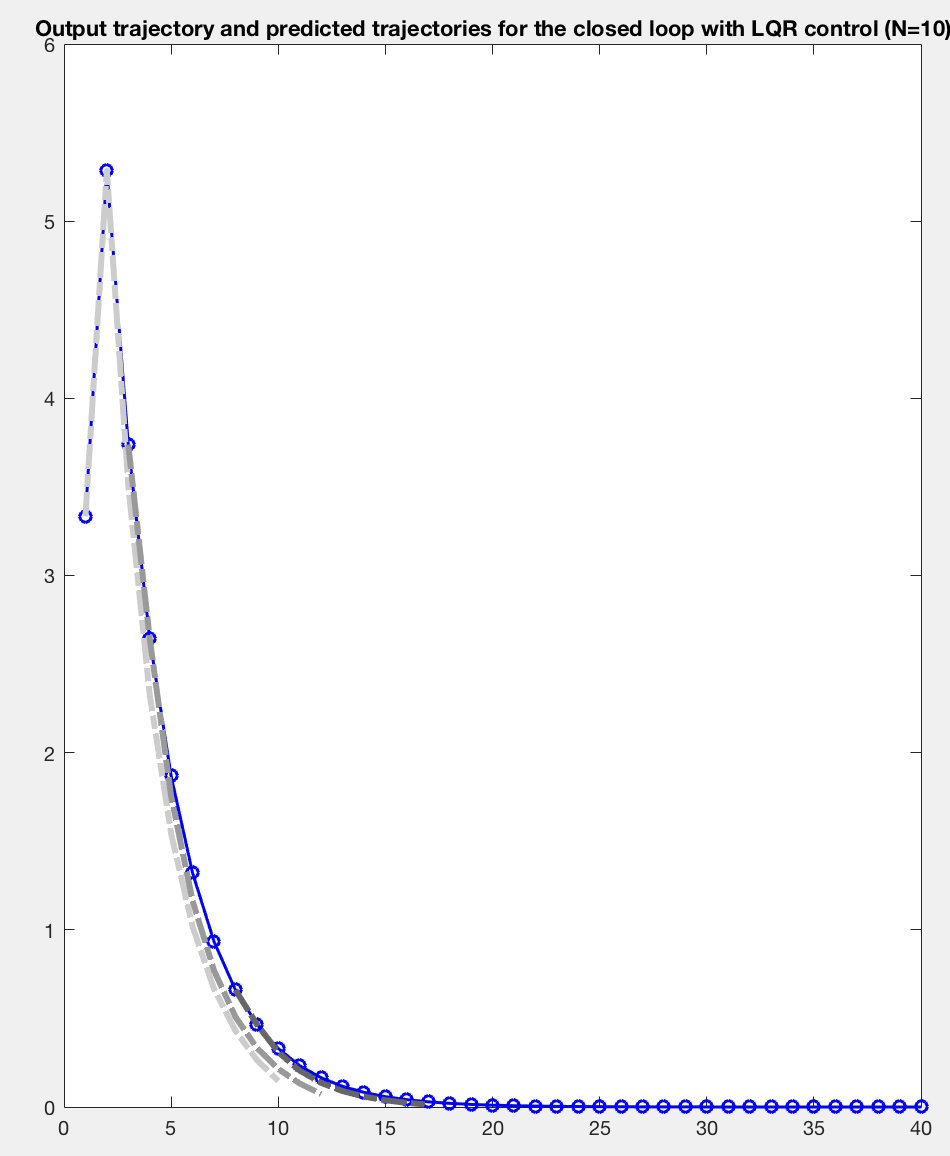
\includegraphics[width=0.9\linewidth]{pred_n10}
				\captionsetup{justification=centering,margin=0.5cm}
				\caption{Predicted and actual output trajectory for N=10}	
				\label{n10}			
			\end{minipage}
		\end{figure}
		
		\paragraph{} Also, \emph{as illustrated in the course}, there are \fbox{no result proving that if the horizon $N^*$ stabilizes the system}, \fbox{than for any horizon $N>N^*$, the system will be stabilized}. 
	}
	
	
		\section{Exercise 3}
	{
		\paragraph{}For this exercise, infinite LQR solutions for $K_{\infty}$ the state feedback law and $P$, the Bellman equation solution were provided by Matlab function \textbf{dlqr}.  Figure (\ref{inf_lqr}) shows the output trajectory and control sequence for the infinite horizon LQR. 
		Figure ({\ref{costs}}) shows cost evolution for infinite horizon LQR ($V_{\infty}(x) = x^TPx$) and LQR with horizon $N^*=7$. We can see that cost value is bigger for infinite LQR in the beginning, this is due to the fact that the evaluated cost takes an infinity of states and control into account to evaluate the cost against only 7 for the other curve. However, infinite LQR cost function decreases much faster since the actual followed trajectory is the optimal one which is not the case for the controller with $N^*=7$. This explains the fact that after a few steps only, the cost function value for infinite LQR gets smaller.
		
			\begin{figure}[h!]
			\begin{minipage}{0.5\linewidth}
				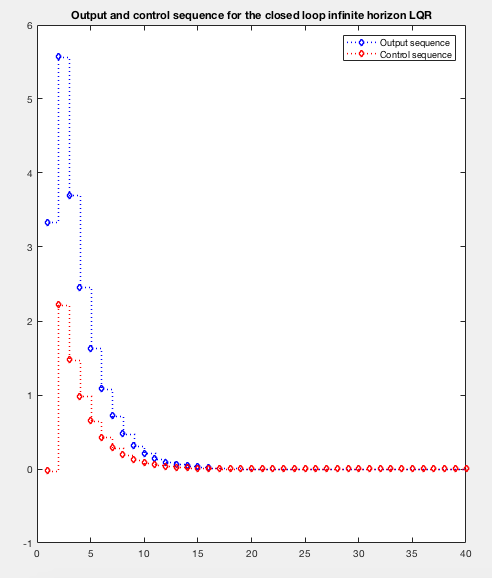
\includegraphics[width=0.9\linewidth]{inf_lqr}
				\captionsetup{justification=centering,margin=0.5cm}
				\caption{Output and control sequences for infinite horizon LQR}
				\label{inf_lqr}
			
			\end{minipage}
			\begin{minipage}{0.5\linewidth}
			
				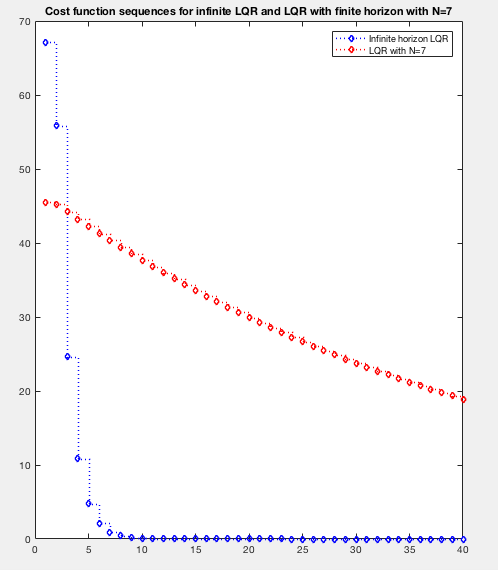
\includegraphics[width=0.9\linewidth]{costs}
				\captionsetup{justification=centering,margin=0.5cm}
				\caption{Cost functions evolution for infinite horizon LQR and LQR with N=7}	
				\label{costs}			
			\end{minipage}
			\end{figure}
		
	
	}

\end{document}